\documentclass{beamer}
\usepackage{ctex, hyperref, fontspec}
\usepackage[T1]{fontenc}

% other packages
\usepackage{latexsym,amsmath,xcolor,multicol,booktabs,calligra}
\usepackage{graphicx,pstricks,listings,stackengine}
\usepackage{caption,array,amssymb}
\usepackage{minted} % code block environment
\usepackage{annotate-equations}
\usepackage{xjtu}

\renewcommand{\eqnannotationfont}{\tiny}

% font and style
\usemintedstyle{manni} % code block style
\usefonttheme[onlymath]{serif} % font in math environment
\setsansfont{PingFang SC} % make sure your system has this font
\setCJKsansfont{STSongti-SC-Bold} % Chinese font, make sure your system has this font

% set background picture
\setbeamertemplate{background}{
  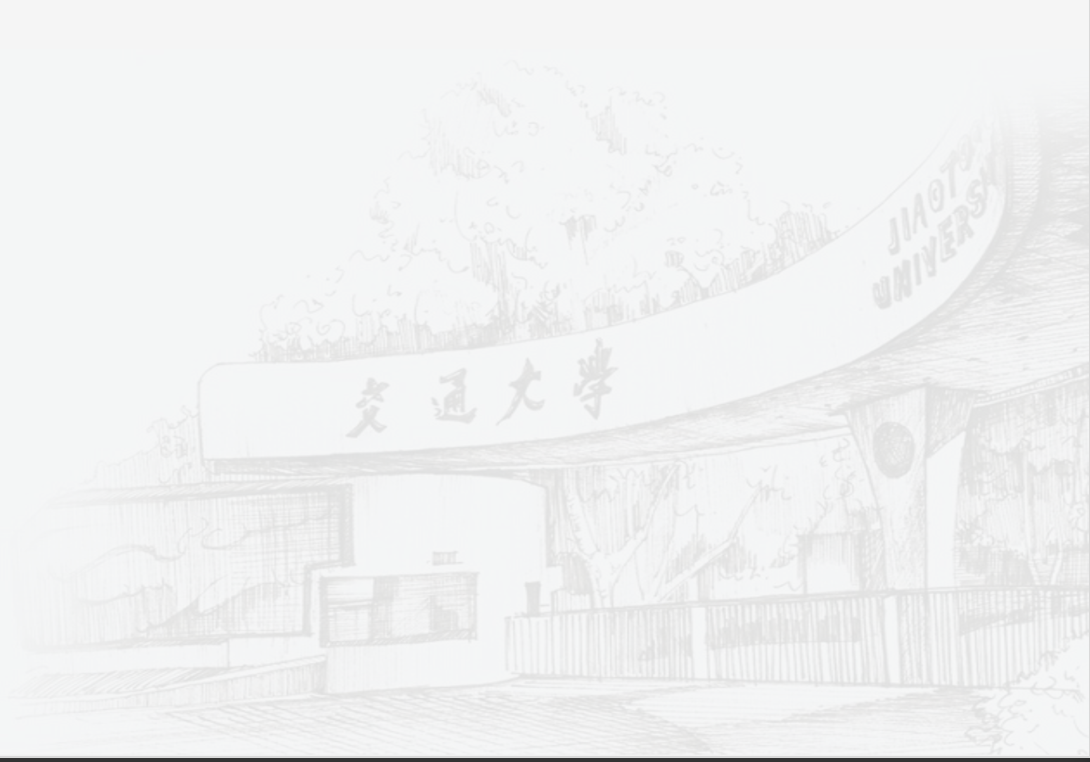
\includegraphics[width=\paperwidth,height=\paperheight]{pic/xjut_draw.png}
}

% natbib settings for "informs2014.bst"
\usepackage{natbib}
 \bibpunct[, ]{(}{)}{,}{a}{}{,}%
 \def\bibfont{\tiny}%
 \def\bibsep{\smallskipamount}%
 \def\bibhang{24pt}%
 \def\newblock{\ }%
 \def\BIBand{and}%

\author{Paramveer S. Dhillon, Sinan Aral}
\title{Modeling Dynamic User Interests: A Neural Matrix Factorization Approach}
% \subtitle{MARKETING SCIENCE}
\institute{MARKETING SCIENCE 2021}
\date{\zhtoday}

% defs
\def\cmd#1{\texttt{\color{red}\footnotesize $\backslash$#1}}
\def\env#1{\texttt{\color{blue}\footnotesize #1}}
\definecolor{deepblue}{rgb}{0,0,0.5}
\definecolor{deepred}{rgb}{0.6,0,0}
\definecolor{deepgreen}{rgb}{0,0.5,0}
\definecolor{halfgray}{gray}{0.55}

\lstset{
    basicstyle=\ttfamily\small,
    keywordstyle=\bfseries\color{deepblue},
    emphstyle=\ttfamily\color{deepred},    % Custom highlighting style
    stringstyle=\color{deepgreen},
    numbers=left,
    numberstyle=\small\color{halfgray},
    rulesepcolor=\color{red!20!green!20!blue!20},
    frame=shadowbox,
}

\begin{document}

\begin{frame}
	\titlepage
	\begin{figure}[htpb]
		\begin{center}
			
\includegraphics[width=0.2\linewidth]{pic/XJUT_Logo.png}
		\end{center}
	\end{figure}
\end{frame}

\begin{frame}
	\tableofcontents[sectionstyle=show,subsectionstyle=show/shaded/hide,subsubsectionstyle=show/shaded/hide]
\end{frame}

\section{Introduction}

\begin{frame}
	\frametitle{Background}
	\begin{itemize}
		\item[$\circledcirc$] 消费者数据(消费者行为数据和UGC)被用于营销领域的各类研究中;
		\item[$\circledcirc$] 三大挑战:
		      \begin{itemize}
			      \item 高维稀疏的非结构化数据, 使用传统方法进行统计推断往往比较困难;
			      \item 数据生成过程本身的非平稳性(动态性);
			      \item 不同于市场营销研究中常见的购买数据建模研究,用户内容消费数据的建模更加复杂,内容消费的种类总是在不断增加,而且几乎没有重复的“动机”。
		      \end{itemize}
	\end{itemize}
\end{frame}

\begin{frame}{Research Question and Objective}
	\begin{itemize}
		\item[$\circledcirc$] 本文旨在解决上述三大挑战,提出了一种基于神经网络的矩阵分解模型,用于建模用户的动态兴趣;
		\item[$\circledcirc$] 模型结果具有可解释性,同时还保留了神经网络的灵活性。
	\end{itemize}

\end{frame}

\section{Related Work}

\begin{frame}{Related Work}
	\begin{itemize}
		\item[$\circledcirc$] 消费者行为建模
		      \begin{itemize}
			      \item 使用Topic Model对用户消费的文本数据进行建模,从而生成用户画像(Trusov et al. 2016).
		      \end{itemize}
		\item[$\circledcirc$] 消费者偏好演变及其对各种营销变量敏感性
		      \begin{itemize}
			      \item 指数平滑模拟品牌偏好的演变(Guadagni and Little 1983);
			      \item 高斯过程模拟消费者偏好的动态变化(Dew et al. 2020);
			      \item 使用粒子滤波对广告和销售等其他营销变量之间的非线性关系进行建模(Bruce 2008)
		      \end{itemize}
		\item[$\circledcirc$] 市场营销领域使用机器学习方法研究客户兴趣(Netzer et al. 2012, Tirunillai and Tellis 2014, B¨uschken and Allenby 2016, Liu and Toubia 2018, Timoshenko and Hauser 2019)
		\item[$\circledcirc$] 矩阵分解
	\end{itemize}
\end{frame}

\section{Model}

\begin{frame}
	\frametitle{Notation}
	\begin{itemize}
		\item[$\circledcirc$] $n$ users, $T$ time slices;
		\item[$\circledcirc$] Content consumed by user $i$ in time period $t$ and user $i$'s unique identity:
		      \begin{equation*}
			      \mathbf{z}_{i}^{t} = \left[\eqnmarkbox[blue]{content}{\mathbf{x}_{i}^{t}} ;\eqnmarkbox[blue]{identity}{\mathbf{a}_{i}}\right]
		      \end{equation*}
		      \annotate[yshift=-0.5em]{below,left}{content}{$p\times 1$ one-hot vector}
		      \annotate[yshift=-0.5em]{below,right}{identity}{$n\times 1$ vector}
		\item[$\circledcirc$]  All content consumed by all users during the whole time slices:
		      \begin{equation*}
			      \eqnmark[blue]{all-content}{\{\mathbf{Z}\}^{t=1: \tau}}
		      \end{equation*}
		      \annotate[yshift=-0.5em]{below}{all-content}{$n\times (n+p)$}
	\end{itemize}
\end{frame}

\begin{frame}[allowframebreaks]{Matrix Factorization for Modeling Users' Content Interests}
	\begin{itemize}
		\item[$\circledcirc$] Approximate the data matrix using the user and content factors
		      \begin{equation*}
			      z_{i j}^t \approx \eqnmarkbox[blue]{item-vec}{v_j}^{\top} \eqnmarkbox[blue]{user-vec}{u_i^t}
		      \end{equation*}
		      \annotate[yshift=-0.5em]{below,left}{item-vec}{$K\times (n+p)$ item vector}
		      \annotate[yshift=-0.5em]{below,right}{user-vec}{$K\times n$ user vector}
		\item[$\circledcirc$] Loss function $\mathcal{L}(\cdot)$
		      \begin{align*}
			      \left(U^t, V\right)&=\underset{U^t, V}{\operatorname{argmin}} \mathcal{L}\left(Z^t, V^{\top} U^t\right) \\
			      &=\left\|Z^t-V^{\top} U^t\right\|_2^2
		      \end{align*}
		\item[$\circledcirc$] Probabilistic form
		      \begin{align*}
			      \begin{aligned}
				      p\left(Z^t \mid U^t, V, \sigma^2\right) & =\prod_{i=1}^n \prod_{j=1}^{p+n} \mathcal{N}\left(z_{i j}^t \mid v_j^{\top} u_i^t, \sigma^2\right), \\
				      p\left(U \mid \sigma_u^2\right) & =\prod_{i=1}^n \mathcal{N}\left(u_i^t \mid 0, \sigma_u^2\right), \\
				      p\left(V \mid \sigma_v^2\right) & =\prod_{j=1}^{p+n} \mathcal{N}\left(v_j \mid 0, \sigma_v^2\right) .
			      \end{aligned}
		      \end{align*}
		      \begin{align*}
			      \begin{aligned}
				      \left(U^t, V\right)= & \underset{U^t, V}{\operatorname{argmin}} \sum_{i=1}^n \sum_{j=1}^{p+n}\left\|z_{i j}^t-v_j^{\top} u_i^t\right\|_2^2+\eqnmarkbox[blue]{lambda-U}{\lambda_U} \sum_{i=1}^n\left\|u_i^t\right\|_2^2 \\
				      & +\eqnmarkbox[blue]{lambda-V}{\lambda_V} \sum_{j=1}^{p+n}\left\|v_j\right\|_{2^{\prime}}^2
			      \end{aligned}
		      \end{align*}
		      \annotate[yshift=-1em]{below,right}{lambda-U}{$\sigma^2 / \sigma_U^2$}
		      \annotate[yshift=-0.5em]{below,left}{lambda-V}{$\sigma^2 / \sigma_V^2$}

		\item[$\circledcirc$] 扩展了基础的矩阵分解模型
		      \begin{itemize}
			      \item 加入非线性因素\citep{trusov2016crumbs};
			      \item 考虑用户潜在因子的状态依赖关系;
			      \item 将矩阵分解框架应用于文本建模任务中。
		      \end{itemize}
	\end{itemize}
	\begin{align*}
		\begin{aligned}
			{\left[\{U\}^{t=1: \tau}, V, \Theta\right] } & =\underset{\{U\}^{t=1: \tau}, V, \Theta}{\operatorname{argmin}} \sum_{i=1}^n \sum_{j=1}^{p+n} \sum_{t=1}^\tau\left\|z_{i j}^t-\eqnmarkbox[red]{mathrm-g}{\mathrm{g}}\left(v_j^{\top} \eqnmarkbox[blue]{u-i-t-1}{u_i^t} ; \Theta\right)\right\|_2^2 \\
			& +\lambda_U \sum_{i=1}^n \sum_{t=1}^\tau\left\|\eqnmarkbox[blue]{u-i-t-2}{u_i^t}\right\|_2^2+\lambda_V \sum_{j=1}^{p+n}\left\|v_j\right\|_2^2
		\end{aligned}
	\end{align*}
	\annotate[yshift=1em]{left}{mathrm-g}{$\mathrm{g}(\cdot)$ encodes the neural network parameterized by $\Theta$}
	\annotate[yshift=-1em]{below,left}{u-i-t-2}{$u_i^t=f\left(u_i^{t-1}\right)$}

\end{frame}

\begin{frame}[allowframebreaks]{Neural Network Architecture}
	\begin{align*}
		\begin{aligned}
			{\left[\{U\}^{t=1: \tau}, V, \Theta\right] } & =\underset{\{U\}^{t=1: \tau}, V, \Theta}{\operatorname{argmin}} \sum_{i=1}^n \sum_{j=1}^{p+n} \sum_{t=1}^\tau\left\|z_{i j}^t-\eqnmarkbox[blue]{mathrm-g}{\mathrm{g}}\left(v_j^{\top} \eqnmarkbox[red]{u-i-t-1}{u_i^t} ; \Theta\right)\right\|_2^2 \\
			& +\lambda_U \sum_{i=1}^n \sum_{t=1}^\tau\left\|\eqnmarkbox[red]{u-i-t-2}{u_i^t}\right\|_2^2+\lambda_V \sum_{j=1}^{p+n}\left\|v_j\right\|_2^2
		\end{aligned}
	\end{align*}
	\annotate[yshift=1em]{left}{mathrm-g}{$\mathrm{g}(\cdot)$ encodes the neural network parameterized by $\Theta$}
	\annotate[yshift=-1em]{below,left}{u-i-t-2}{$u_i^t=f\left(u_i^{t-1}\right)$}

	\pagebreak
	\begin{itemize}
		\item[$\circledcirc$] Embedding the Input Data
		      \begin{align*}
			      \left\{x_i^t, a_i\right\} \rightarrow \left\{\eqnmarkbox[blue]{E-x}{E_{x}}x_{i}^{t},\eqnmarkbox[blue]{E-a}{E_{a}}a_{i}\right\}
		      \end{align*}
		      \annotate[yshift=-0.5em]{below,left}{E-x}{$d\times p$}
		      \annotate[yshift=-0.5em]{below,right}{E-a}{$d\times n$}
		      \annotate[yshift=0.5em]{right}{E-a}{model parameter}
		      \annotate[yshift=0.5em]{left}{E-x}{pretrained embeddings}
		\item[$\circledcirc$] Estimating a Nonlinear Hidden State for Each User
		      \begin{align*}
			      \ell_i^t=\eqnmarkbox[red]{sigma-1}{\sigma_1}\left(\eqnmarkbox[blue]{W-l}{W_{\ell}} \cdot\left[E_x x_i^t ; E_a a_i\right]\right)
		      \end{align*}
		      \annotate[yshift=-0.5em]{below,left}{sigma-1}{ReLU}
		      \annotate[yshift=-0.5em]{below,right}{W-l}{$d\times 2d$}
		      \pagebreak
		\item[$\circledcirc$] Incorporating Dynamics by Combining a User’s Current and Previous Hidden States
		      \begin{align*}
			      u_i^t=\eqnmarkbox[red]{sigma-2}{\sigma_2}\left(\eqnmarkbox[blue]{W-u}{W_{u}}\ell_{i}^{t} + \eqnmarkbox[blue]{W-r}{W_{r}}u_{i}^{t-1}\right)
		      \end{align*}
		      \annotate[yshift=-0.5em]{below,left}{sigma-2}{softmax}
		      \annotate[yshift=-0.5em]{below,right}{W-u}{$K\times d$}
		      \annotate[yshift=0.5em]{right}{W-r}{$K\times K$}
		      \begin{align*}
			      u_i^t=\eqnmarkbox[red]{alpha}{\alpha} \cdot\left[\sigma_2\left(W_u \ell_i^t+W_r u_i^{t-1}\right)\right]+(1-\alpha) \cdot u_i^{t-1}
		      \end{align*}
		      \annotate[yshift=-0.5em]{below,right}{alpha}{smoothing hyperparameter}
		\item[$\circledcirc$] Combining the User and Content Factors (Encoder-decoder architecture)
		      \begin{align*}
			      r_i^t=\eqnmarkbox[blue]{V}{V}^{\top} u_i^t
		      \end{align*}
		      \annotate[yshift=-0.5em]{below,right}{V}{$K\times d$}
		\item[$\circledcirc$] Minimizing the Loss Function
		      \begin{align*}
			      \left[\{U\}^{t=1: \tau}, V\right]=\underset{U^{t=1: \tau}, V}{\operatorname{argmin}} \sum_{i=1}^n \sum_{t=1}^\tau\left\|E_x x_i^t-r_i^t\right\|_2^2
		      \end{align*}
		\item[$\circledcirc$] Hyperparameters: $K=30,\alpha=0.5,d=300$, random uniform initialization.
	\end{itemize}

	\begin{figure}[htpb]
		\centering
		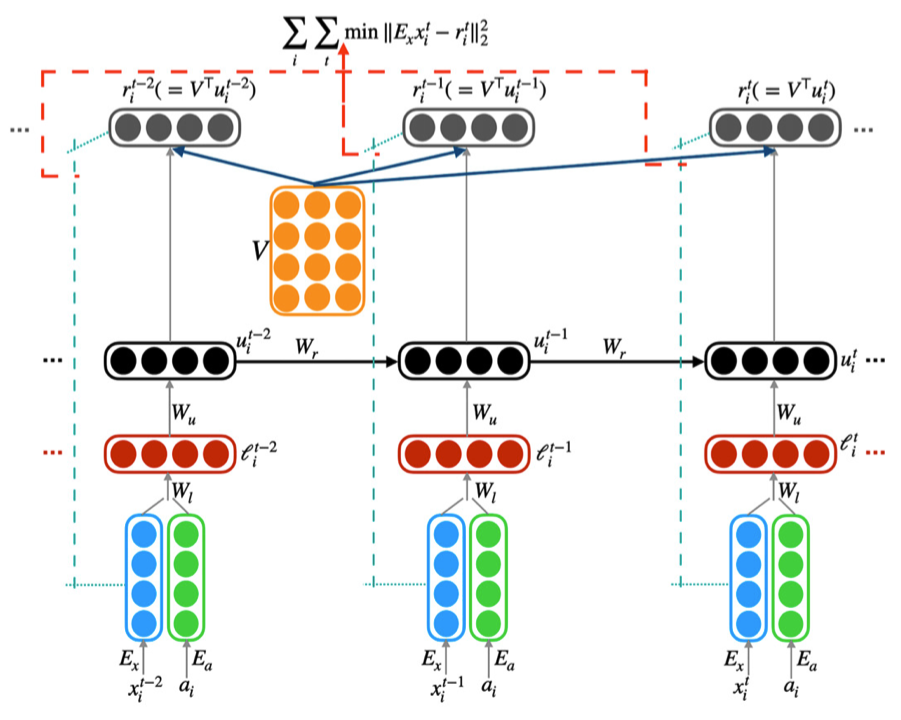
\includegraphics[width=0.6\textwidth]{pic/nn-arch.png}
	\end{figure}
\end{frame}

\section{Data}

\begin{frame}[allowframebreaks]{Data}
	\begin{itemize}
		\item[$\circledcirc$] 《波士顿环球报》2014年2月1日-2019年5月13日的用户点击流数据;
		\item[$\circledcirc$] 阅读的文章、阅读文章的时长、订阅状态、访问者的人口统计数据: 如地区代码、邮政编码、设备类型(手机或台式机)、操作系统和国家;
		\item[$\circledcirc$] Week level analysis;
		\item[$\circledcirc$] Visit the website at least five different times;
		\item[$\circledcirc$] 500000 unique visitors over 276 weeks, 5610008 non-zero person-week observations;
		\item[$\circledcirc$] Use headlines, 135861569 tokens, 85228 unique tokens;
	\end{itemize}
	\begin{figure}[htpb]
		\centering
		\begin{minipage}[t]{0.45\textwidth}
			\centering
			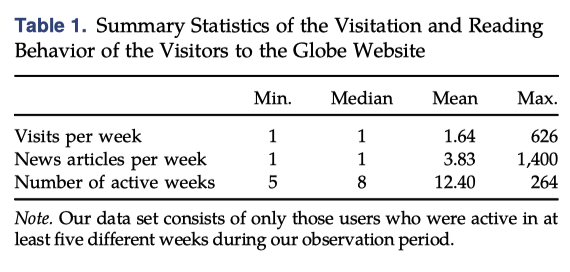
\includegraphics[width=\textwidth]{pic/behavior-data.png}
		\end{minipage}
		\begin{minipage}[t]{0.45\textwidth}
			\centering
			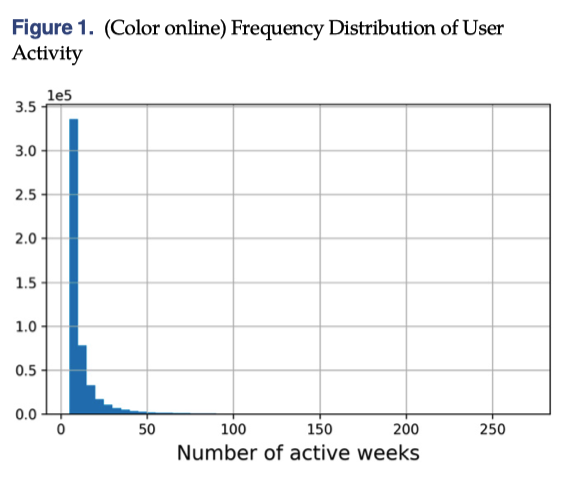
\includegraphics[width=\textwidth]{pic/freq-week.png}
		\end{minipage}
	\end{figure}

	\begin{figure}[htpb]
		\centering
		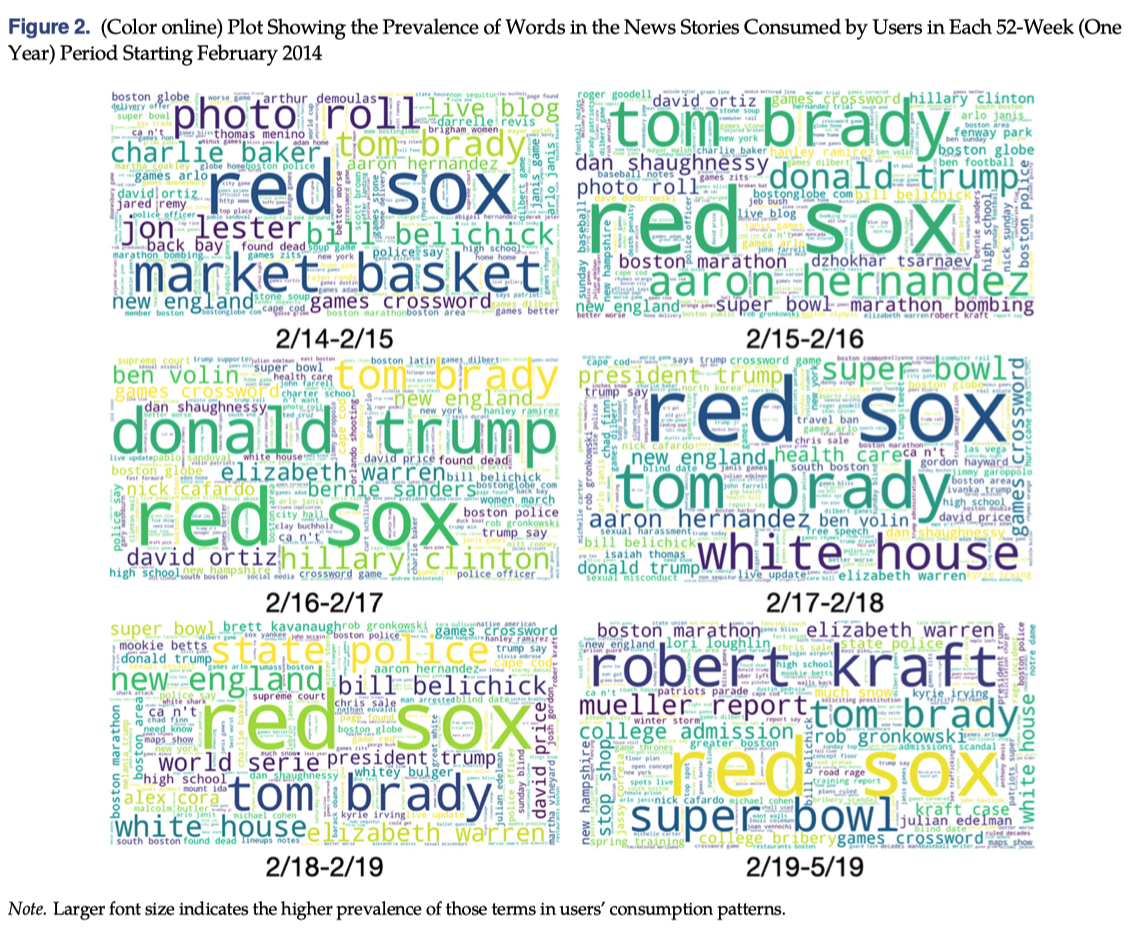
\includegraphics[width=0.75\textwidth]{pic/tokens.png}
	\end{figure}
\end{frame}

\section{Results}

\begin{frame}{Visualizing Trajectories of User Interests $U^{t}$}
	Compute the nearest neighbors of each row of $V$ from the word embedding matrix $E_x$.
	\begin{figure}[htpb]
		\centering
		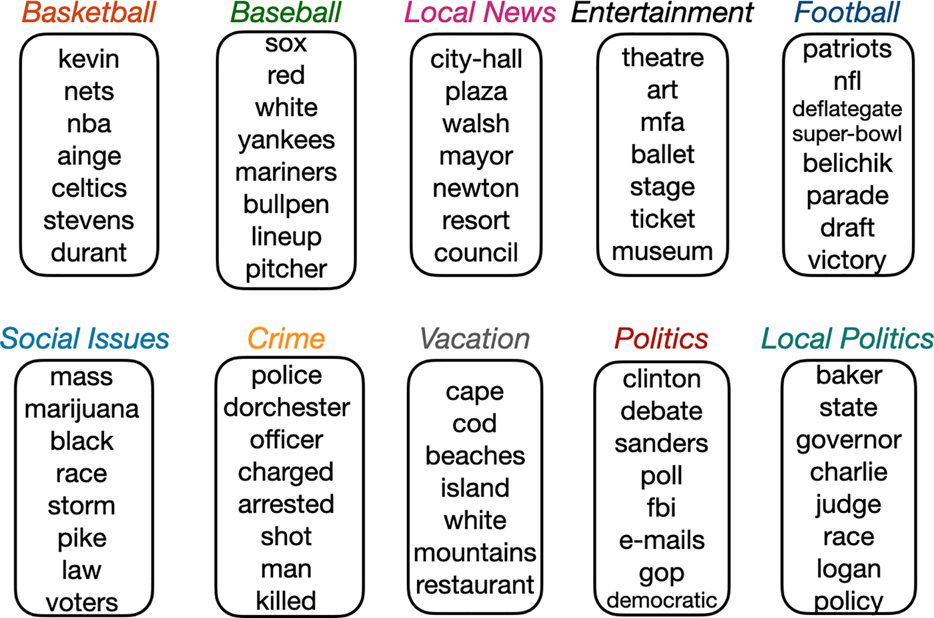
\includegraphics[width=0.7\textwidth]{pic/word-dist.png}
	\end{figure}
\end{frame}

\begin{frame}{Stable Interests}
	\begin{figure}[htpb]
		\centering
		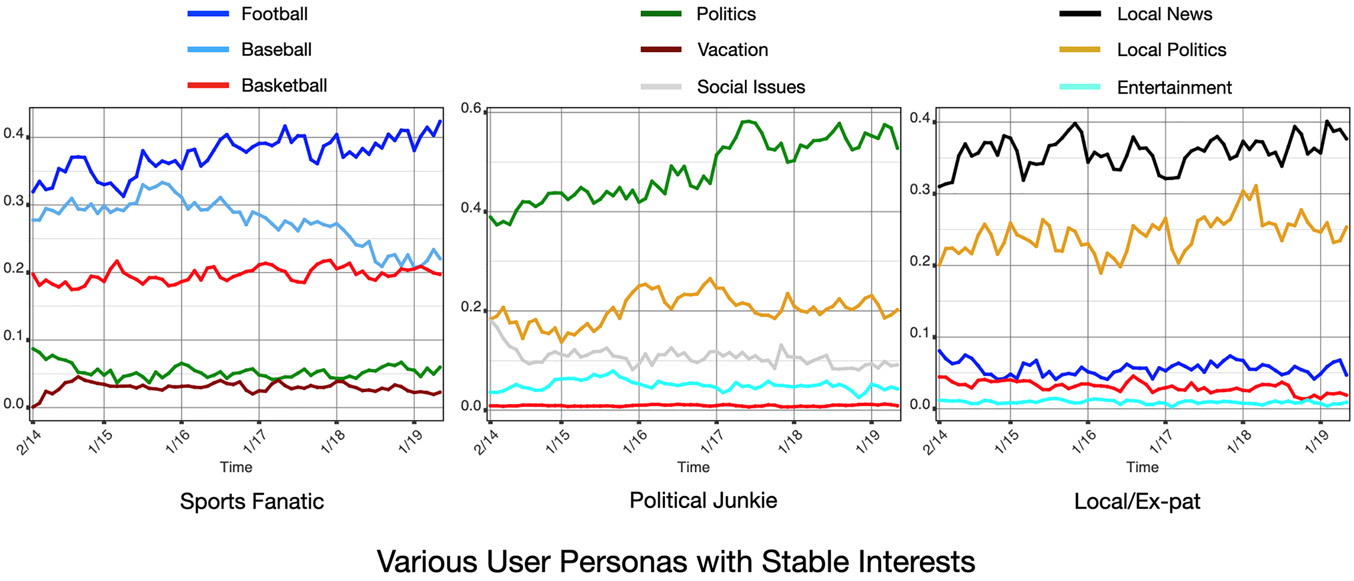
\includegraphics[width=0.8\textwidth]{pic/stable-interests.png}
	\end{figure}
\end{frame}

\begin{frame}{Evolving Interests}
	\begin{figure}[htpb]
		\centering
		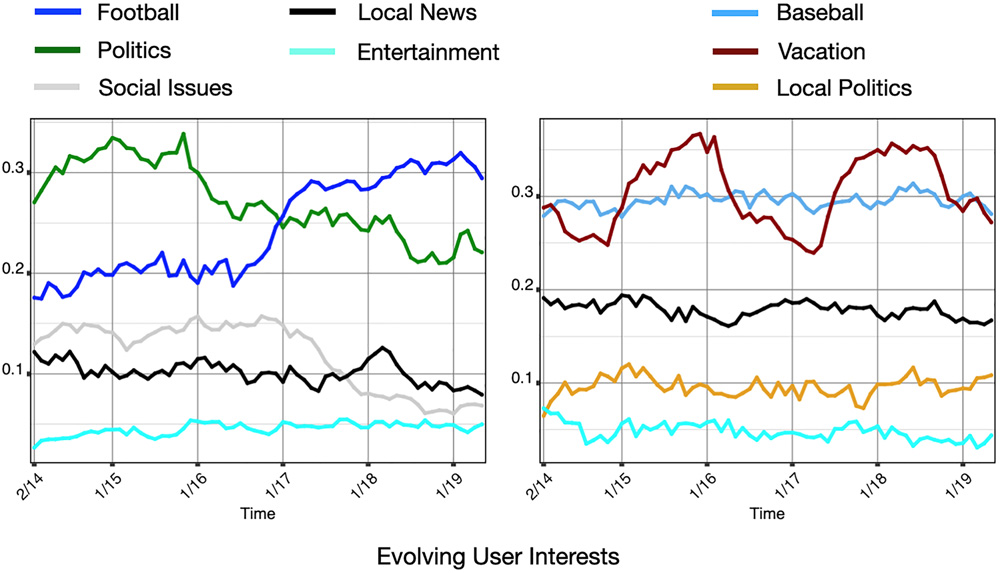
\includegraphics[width=0.8\textwidth]{pic/evolving-interests.png}
	\end{figure}
\end{frame}

\begin{frame}[allowframebreaks]{Crowdsourced Evaluation of Content Attributes}
	\begin{itemize}
		\item[$\circledcirc$]  Word intrusion task
		\item[$\circledcirc$] $K=\{10,30,50,100\}$
		      \begin{align*}
			      \text { Mean Precision }_k=\sum_{s=1}^S \frac{1\left(i_{k, s}=w_k\right)}{S}
		      \end{align*}
	\end{itemize}

	\begin{figure}[htpb]
		\centering
		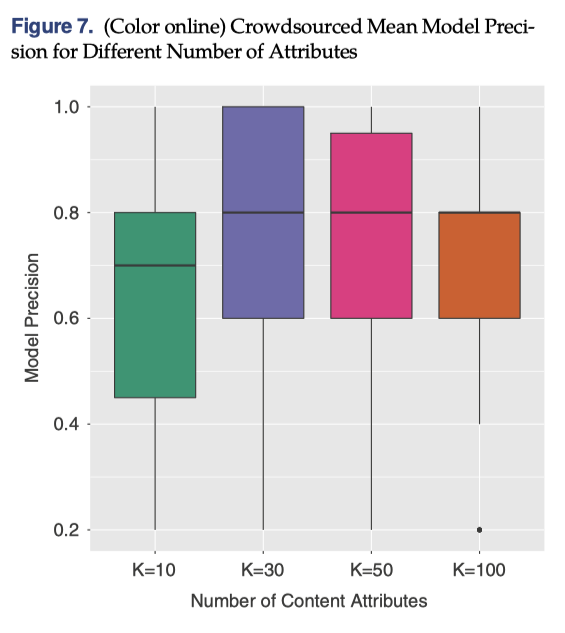
\includegraphics[width=0.5\textwidth]{pic/intrusion-prec.png}
	\end{figure}
\end{frame}

\begin{frame}{Evaluating the Predictive Quality}
	\begin{itemize}
		\item[$\circledcirc$] Mean precision at K (MP@K)
		      \begin{align*}
			      \text { Mean Precision }=\sum_{i=1}^n \frac{1\left(\eqnmarkbox[red]{NN-1}{\mathrm{NN}_1}\left(\eqnmarkbox[blue]{r-i-tau-a}{r_i^{\tau-a}}\right)=\eqnmarkbox[blue]{c-i-tau}{c_i^\tau}\right)}{n}
		      \end{align*}

		\item[$\circledcirc$] Real-valued similarity score $s\left(r_i^{\tau-a}, c_i^\tau\right)$.
	\end{itemize}
	\annotate[yshift=-2em]{below,left}{NN-1}{nearest neighbor function}
	\annotate[yshift=0.5em]{left}{r-i-tau-a}{$t=\tau-a$ representation}
	\annotate[yshift=0.5em]{right}{c-i-tau}{$t=\tau$ representation}
\end{frame}

\begin{frame}{Evaluating the Predictive Quality}
	\begin{figure}[htpb]
		\centering
		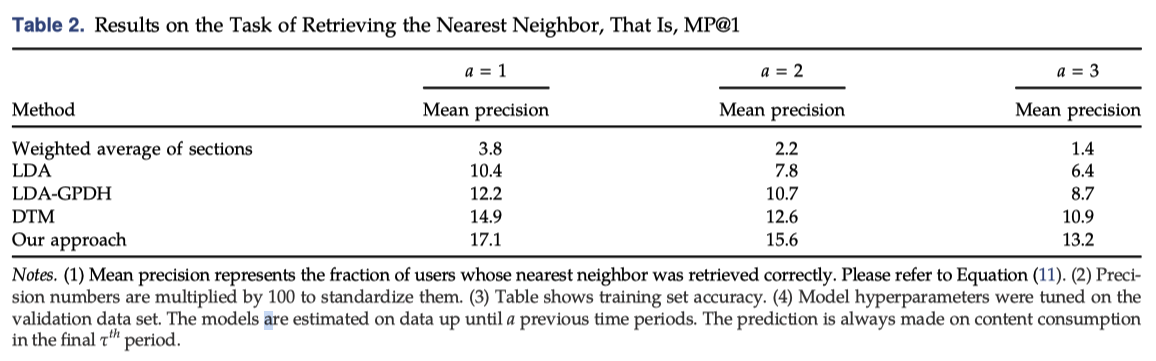
\includegraphics[width=0.7\textwidth]{pic/prediction-eval.png}
	\end{figure}
	\begin{figure}[htpb]
		\centering
		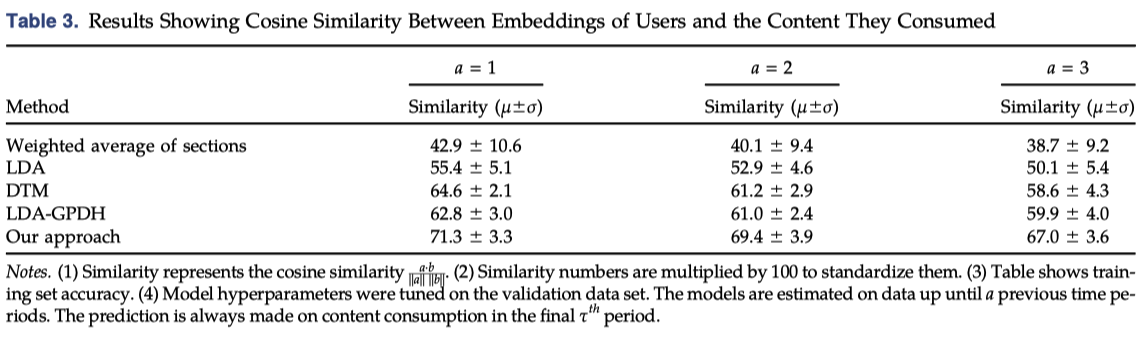
\includegraphics[width=0.7\textwidth]{pic/sim.png}
	\end{figure}
\end{frame}

\begin{frame}{Robustness Tests}
	\begin{figure}[htpb]
		\centering
		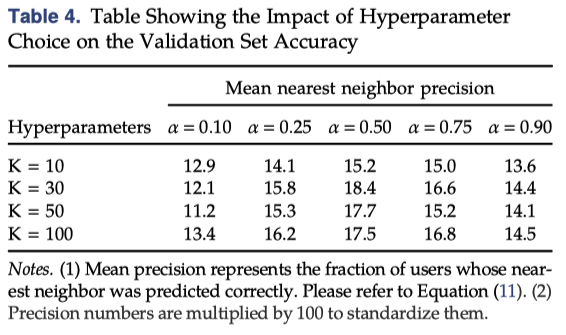
\includegraphics[width=0.6\textwidth]{pic/robustness.png}
	\end{figure}
\end{frame}

\begin{frame}{Ablation Analysis}
	\begin{figure}[htpb]
		\centering
		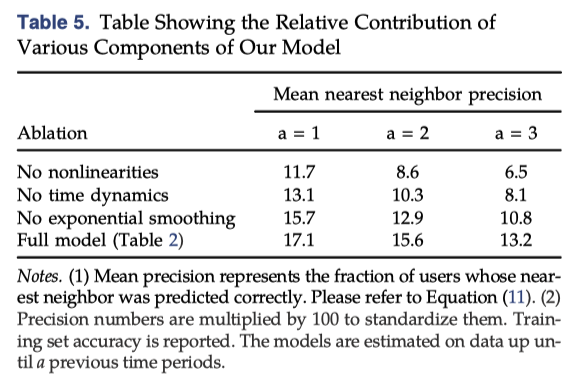
\includegraphics[width=0.6\textwidth]{pic/Ablation.png}
	\end{figure}
\end{frame}

\begin{frame}{Scalability, Transferability, and Cold-Starting New Users.}
	\begin{itemize}
		\item[$\circledcirc$] Use transfer learning to learn representations for users with consumption traces $x_{i}^{t}$.
		\item[$\circledcirc$] Freezing all the estimated parameters: $\left\{W_{\ell}, W_u, W_r, V, E_x\right\}$.
		\item[$\circledcirc$] Use the observable user demographics.
	\end{itemize}
\end{frame}

\section{Discussion}

\begin{frame}{Managerial Implications}
	\begin{itemize}
		\item[$\circledcirc$] Generating User Profiles
		\item[$\circledcirc$] Content Categorization and Recommendation
	\end{itemize}
\end{frame}

\begin{frame}{Conclusion and Limitations}
	\begin{itemize}
		\item[$\circledcirc$] Proposed a neural matrix factorization modeling approach to extract nonlinear patterns from text data to infer customers' evolving interests.
		\item[$\circledcirc$] Model other types of high-dimensional consumption data(e.g., images, videos, and audio).
		\item[$\circledcirc$] Limitations
		      \begin{itemize}
			      \item Model only one kind of customer digital footprints—news consumption;
			      \item Deep learning and neural net models in marketing research is still an under explored area of study;
			      \item Only model the demand side and assume that consumers' consumption patterns are driven only by their consumption in previous periods.
		      \end{itemize}
	\end{itemize}
\end{frame}

% \begin{frame}[fragile]{Code Block Example}
%     \begin{minted}[fontsize=\tiny]{python3}
%         class ProdLDA(nn.Module):
%             def __init__(self, vocab_size, num_topics, hidden, dropout):
%                 super().__init__()
%     \end{minted}
% \end{frame}

\begin{frame}[allowframebreaks]{References}
	\bibliography{reference.bib}
	\bibliographystyle{informs2014}
\end{frame}

\begin{frame}
	\begin{center}
		{\Huge\calligra Thanks!}
	\end{center}
\end{frame}

\end{document}